\documentclass[11pt]{article}
\usepackage{graphicx}
\usepackage{hyperref}
\usepackage{appendix}
\usepackage{amsmath}
\usepackage{amsthm}
\usepackage{amssymb}
\usepackage{natbib}
\usepackage{float}
\usepackage{multirow}
\usepackage{commath}
\usepackage{booktabs}
\usepackage{subcaption}
\renewcommand{\arraystretch}{1.2}
\usepackage{siunitx}
\sisetup{detect-all}
\usepackage{listings}
\usepackage{color} %red, green, blue, yellow, cyan, magenta, black, white
\definecolor{mygreen}{RGB}{28,172,0} % color values Red, Green, Blue
\definecolor{mylilas}{RGB}{170,55,241}
\usepackage[a4paper,margin=20mm]{geometry}
\numberwithin{equation}{section}
\setlength{\parskip}{\baselineskip}
\setlength{\parindent}{0pt}
\hypersetup{
    colorlinks=true,
    linkcolor=black,
    filecolor=black,      
    urlcolor=black,
    citecolor=black
}
\urlstyle{same}
\lstset{language=Matlab,%
    %basicstyle=\color{red},
    breaklines=true,%
    morekeywords={matlab2tikz},
    keywordstyle=\color{blue},%
    morekeywords=[2]{1}, keywordstyle=[2]{\color{black}},
    identifierstyle=\color{black},%
    stringstyle=\color{mylilas},
    commentstyle=\color{mygreen},%
    showstringspaces=false,%without this there will be a symbol in the places where there is a space
    numbers=left,%
    numberstyle={\tiny \color{black}},% size of the numbers
    numbersep=9pt, % this defines how far the numbers are from the text
    emph=[1]{for,end,break},emphstyle=[1]\color{red}, %some words to emphasise
    %emph=[2]{word1,word2}, emphstyle=[2]{style},    
}
\begin{document}
\title{\textbf{UCL Mechanical Engineering 2021/2022}\\MECH0023 Coursework}
\author{RFLH9}
\date{\today}
\maketitle
\tableofcontents
\listoffigures
\section{Satellite model}
\subsection{Description of model and assumptions}
We are given some information about some parameters of the system. They are:
\begin{itemize}
    \item Beam cross-section is rectangular.
    \item Beam width is \SI{5}{\centi\meter}.
    \item Beam material is high-grade aluminium alloy with modulus of elasticity \SI{70}{\giga\pascal}.
    \item Beam length is \SI{1.1}{\meter}.
    \item Sensor weight is \SI{1.2}{\kilo\gram}.
\end{itemize}
Hence, we can begin to start modelling our system. Our first assumption is that the satellite is oscillating only in the $x$-axis as show in Figure \ref{q1a}.
\begin{figure}[H]
    \centering
    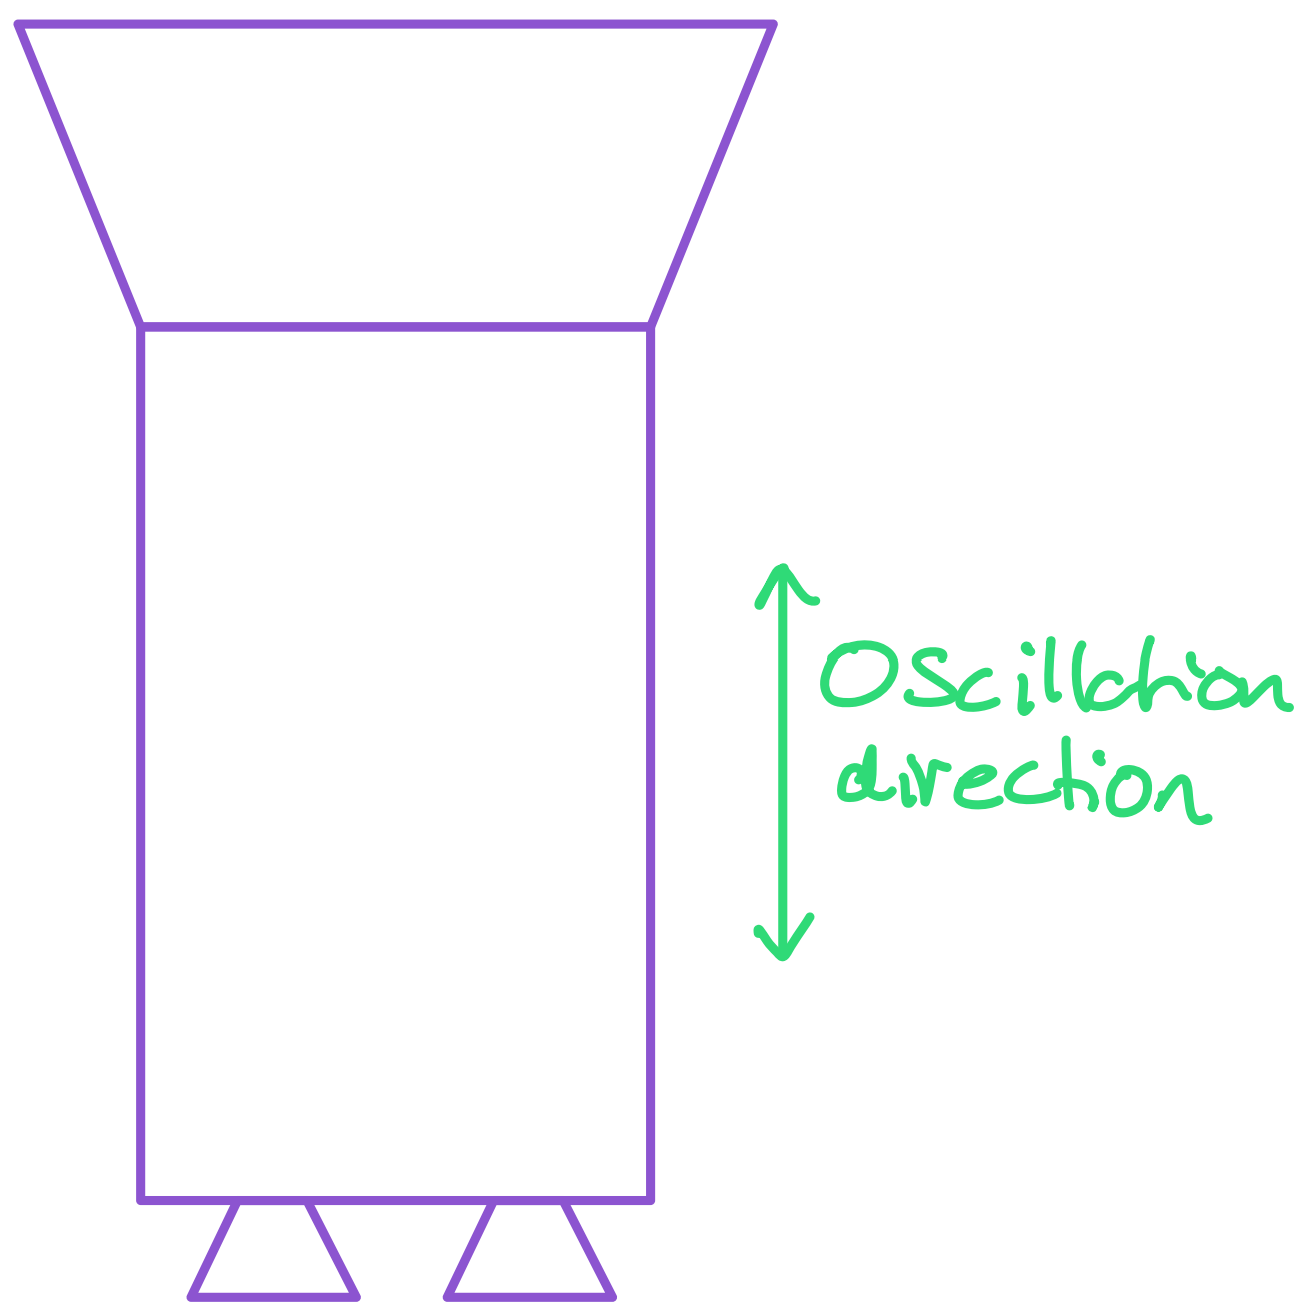
\includegraphics[width = 0.3\textwidth]{./img/q1a.png}
    \caption{Satellite oscillation.}
    \label{q1a}
\end{figure}
We can now simplify our supporting beam to a fixed cantilever beam with a mass at the free end. The vibrating base seen in Figure \ref{q1a2} is in reference to the oscillations that would be transmitted through the satellite frame to the base of the cantilever beam.
\begin{figure}[H]
    \centering
    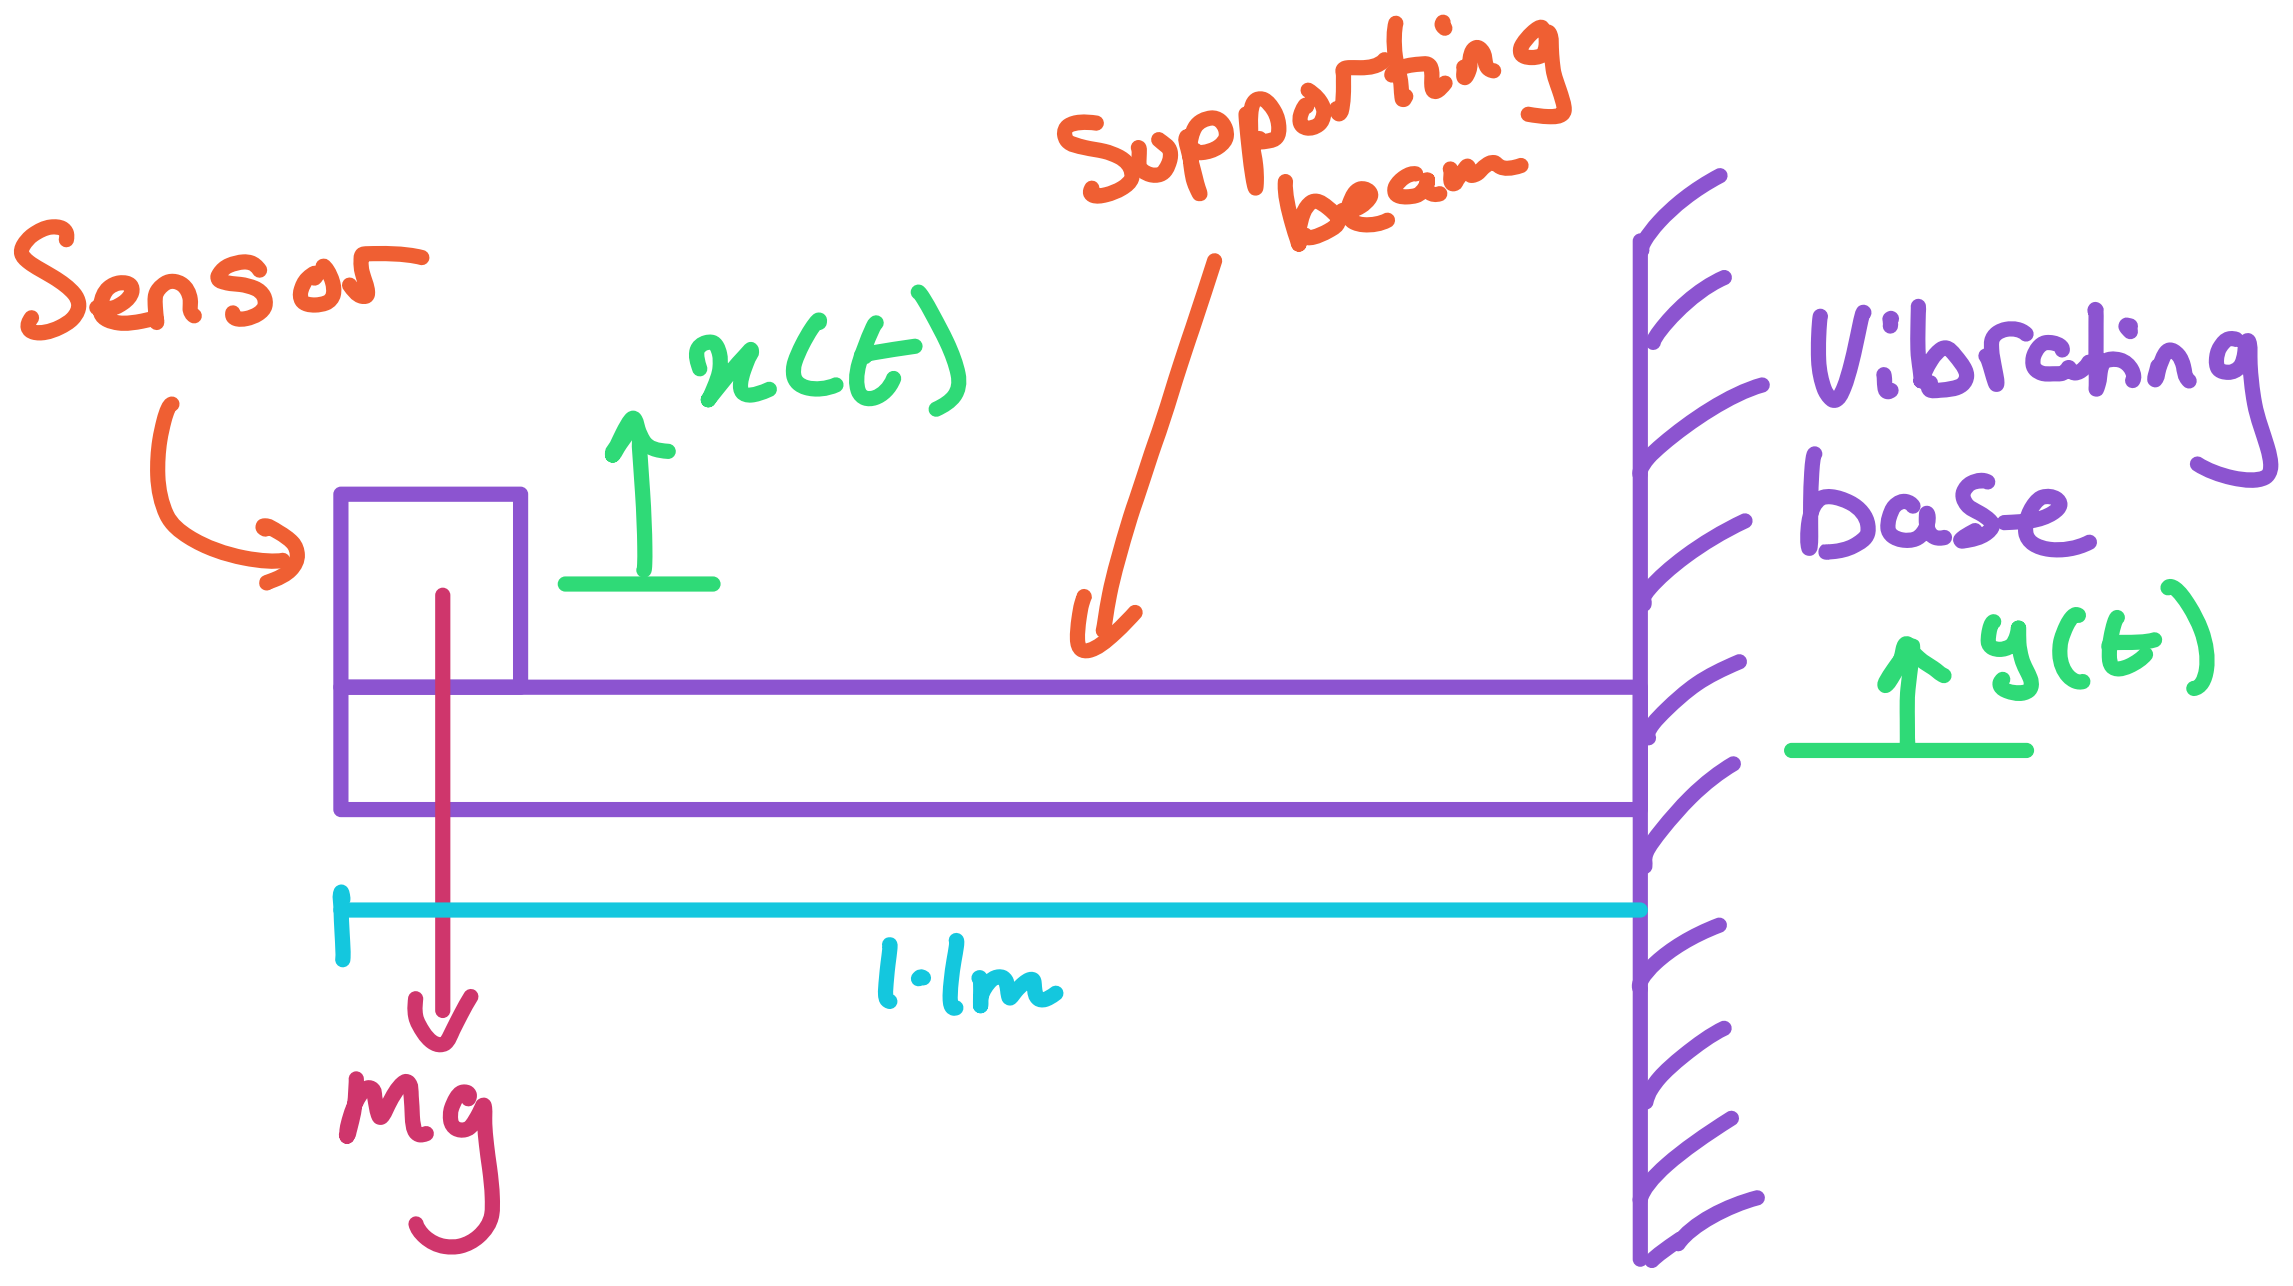
\includegraphics[width = 0.6\textwidth]{./img/q1a2.png}
    \caption{Supporting beam diagram.}
    \label{q1a2}
\end{figure}
Finally, we can model the sensor system as a mass attached to a base via a spring and a damper. As our satellite's environment will drastically change during the course of its journey to space (atmosphere $\rightarrow$ vacuum of space), we will see a change in the way viscous damping (atmospheric drag) will affect our system. We also have frictional losses from the cantilever support and material damping in our system. We can simplify our model by considering the damping force to be constant throughout the operational timeframe of the satellite.
\begin{figure}[H]
    \centering
    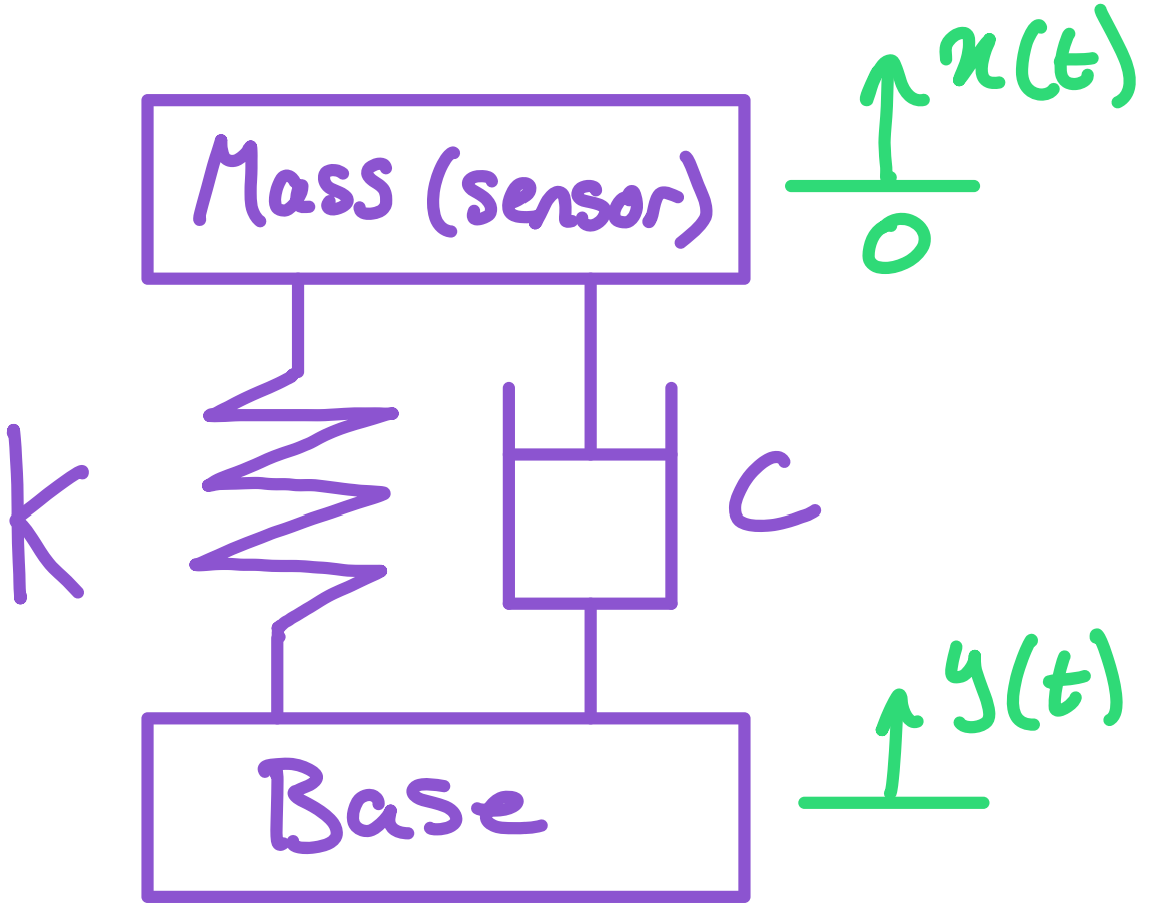
\includegraphics[width = 0.5\textwidth]{./img/q1a3.png}
    \caption{Model of system.}
    \label{q1a3}
\end{figure}
\subsection{Minimum thickness of beam}
\begin{figure}[H]
    \centering
    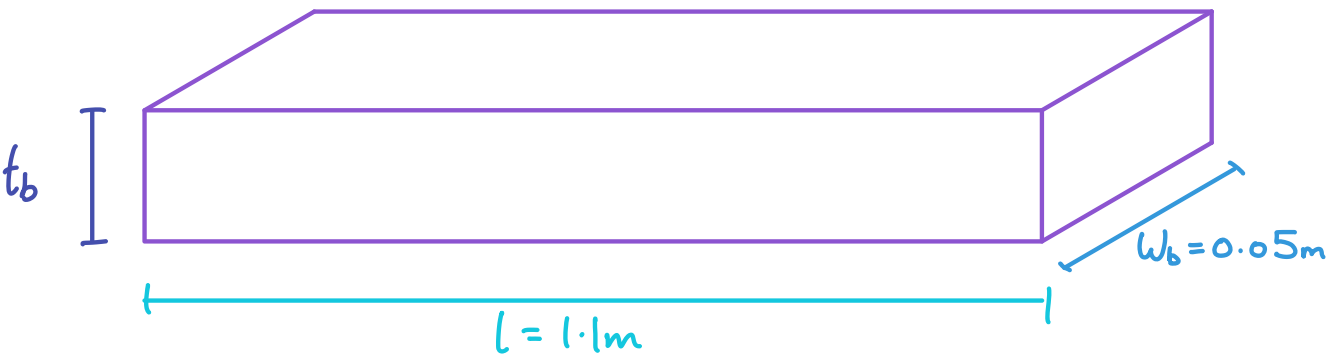
\includegraphics[width = 0.75\textwidth]{./img/q1b.png}
    \caption{Diagram to show beam dimensions.}
    \label{q1b}
\end{figure}
The relative motion of the mass from the base can be set as:
\begin{gather}
    z = x - y\label{eq:q1b.1}
\end{gather}
Next we can look at the equation of motion for the system:
\begin{gather}
    m\ddot{x} + c \left(\dot{x} - \dot{y}\right) + k \left(x- y \right) = 0\label{eq:q1b.2}
\end{gather}
Substituting \ref{eq:q1b.1} into \ref{eq:q1b.2}:
\begin{gather}
    m \ddot{z} + m\ddot{y} + c\dot{z} + kz = 0\label{eq:q1b.3}
\end{gather}
We are given that $\zeta = 0.003$, hence our system is underdamped. The standard solution for \ref{eq:q1b.3} for underdamped conditions is:
\begin{gather}
    z\left(t\right) = Ae^{-\zeta \omega_n t} \sin\left(\omega_d t + \phi\right) \label{eq:q1b.9}
\end{gather}
where:
\begin{align}
    A    & = \frac{\sqrt{\left(\dot{z_0}^2 + \zeta \omega_n z_0 \right)^2 + \left(\omega_d z_0\right)^2}}{\omega_d} \label{eq:q1b.4} \\
    \phi & = \arctan \left(\frac{z_0 \omega_d}{\dot{z_0} + \zeta \omega_n z_0}\right) \label{eq:q1b.5}
\end{align}
Boundary conditions:
\begin{align}
    \dot{z_0}                           & = \SI{0.04}{\meter\per\second} \\
    z_0                                 & = \SI{0}{\meter}               \\
    z\left(t = \SI{900}{\second}\right) & < \SI{0.0001}{\meter}
\end{align}
Inputting boundary conditions into \ref{eq:q1b.4} and \ref{eq:q1b.5}:
\begin{align}
    A    & = \frac{\sqrt{\left(0.04^2 + 0.0003 \cdot \omega_n \cdot 0 \right)^2 + \left(\omega_d \cdot 0 \right)^2}}{\omega_d} \\
    A    & = \frac{0.04}{\omega_d}\label{eq:q1b.6}                                                                             \\
    \phi & = \arctan \left(\frac{0 \cdot \omega_d}{0.04 + 0.0003 \cdot \omega_n \cdot 0}\right)                                \\
    \phi & = 0\label{eq:q1b.7}
\end{align}
We know that:
\begin{align}
    \omega_d = \omega_n \sqrt{1 - \zeta^2} \label{eq:q1b.8}
\end{align}
Substituting \ref{eq:q1b.6}, \ref{eq:q1b.7}, \ref{eq:q1b.8} into \ref{eq:q1b.9}:
\begin{align}
    z\left(t\right) = \dfrac{0.04e^{-\zeta \omega_n t}}{\omega_n \sqrt{1 - \zeta^2}} \sin\left(\omega_n \sqrt{1 - \zeta^2} t\right) \label{eq:q1b.10}
\end{align}
Next, we must determine $\omega_n$, we can find the natural frequency of the cantilever beam with simulated load at free end from our work in the MECH0013 module. The deflection at the free end $\delta_{fe}$ is given by:
\begin{gather}
    \delta_{fe} = \frac{mgl^3}{3EI}
\end{gather}
We also know:
\begin{gather}
    k = \frac{mg}{\delta_{fe}} = \frac{3EI}{l^3}
\end{gather}
Moment of inertia:
\begin{gather}
    I = \frac{w_b t_b^3}{12}
\end{gather}
Therefore:
\begin{gather}
    k = \frac{E w_b t_b^3}{4l^3}
\end{gather}
$k$ is related to the natural frequency through:
\begin{gather}
    \omega_n = \sqrt{\frac{k}{m}}
\end{gather}
Looking at the amplitude term of \ref{eq:q1b.10}, we know this must be less than \SI{0.0001}{\meter} at $t = \SI{900}{\second}$:
\begin{gather}
    \dfrac{0.04e^{-\zeta \omega_n t}}{\omega_n \sqrt{1 - \zeta^2}} < 0.0001
\end{gather}
Solving:
\begin{gather}
    \dfrac{0.04}{\sqrt{\dfrac{E w_b t_b^3}{4l^3m}} \sqrt{1 - \zeta^2}} \cdot e^{-\zeta \sqrt{\dfrac{E w_b t_b^3}{4l^3m}} t}                                                                                                                     < 0.0001 \label{eq:q1b.11} \\
    \dfrac{0.04}{\sqrt{\dfrac{70\cdot 10^9 \cdot 0.05\cdot  t_b^3}{4\cdot 1.1^3\cdot 1.2}} \sqrt{1 - 0.003^2}}\cdot  e^{\left(-0.003 \sqrt{\dfrac{70\cdot 10^9 \cdot 0.05\cdot  t_b^3}{4\cdot 1.1^3\cdot 1.2}} \cdot 900\right)}  < 0.0001
\end{gather}
The result was inputted into MATLAB and a numerical answer for $t_b$ was obtained. The MATLAB code used is below.
\lstinputlisting{./mCode/q1b.m}
This generated the plot shown in Figure \ref{q1b2}
\begin{figure}[H]
    \centering
    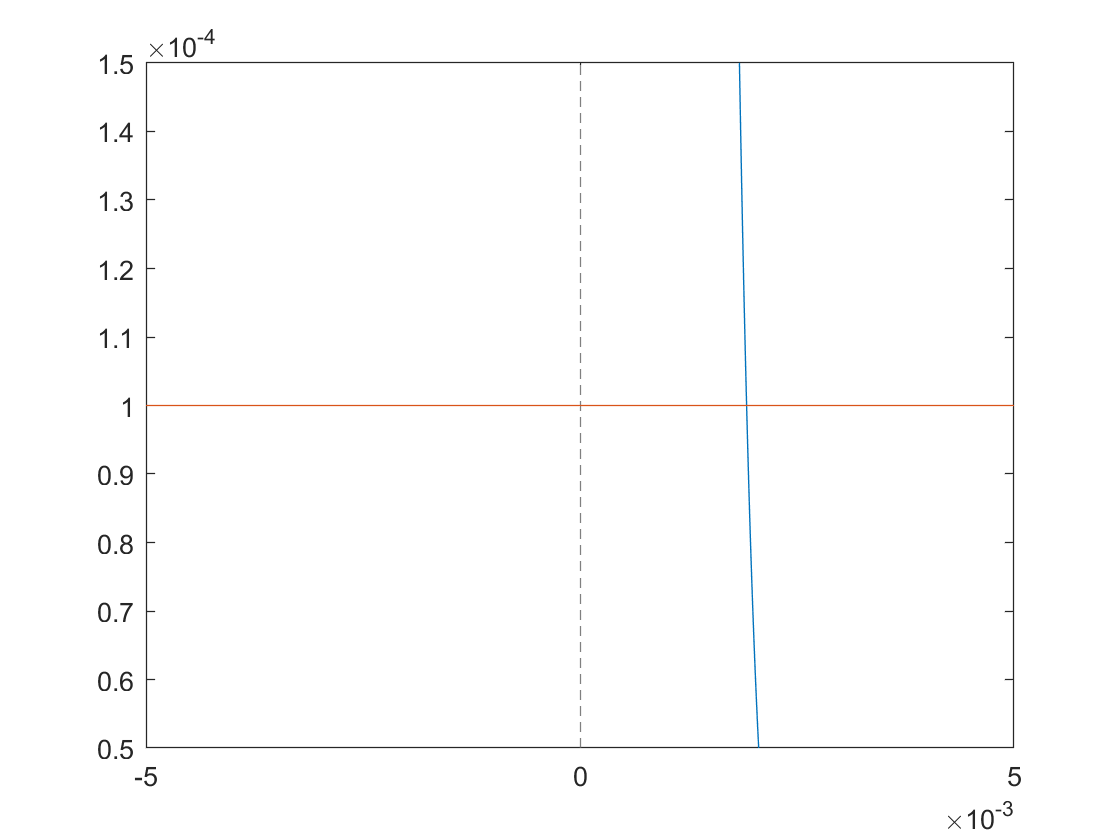
\includegraphics[width = 0.5\textwidth]{./img/q1b2.png}
    \caption{Plot to show \ref{eq:q1b.11}.}
    \label{q1b2}
\end{figure}
Using MATLAB's \lstinline{vpasolve} function, we can numerically solve our equation. This function can take an \lstinline{init_param} variable. This allows MATLAB to solve for values close to the variable. By visually observing the plot, we can see that our solution is in the vicinity of 0.001. Hence, this was chosen as the initial parameter. This yielded:
\begin{gather}
    t_b \approx \SI{0.00192}{\meter}\\
    t_b \approx \SI{1.92}{\milli\meter}
\end{gather}
\subsection{Amplitude of displacement for steady-state oscillation of the sensor during rocket function}
This is a case of base excitation. The equation to describe the motion of our base excitation takes the standard form:
\begin{gather}
    y(t) = Y\sin\left(\omega t\right)\label{eq:q1c.1}
\end{gather}
Therefore:
\begin{gather}
    m \ddot{x} + c\left(\dot{x} - \dot{y}\right) + k\left(x-y\right)=0\\
    m\ddot{x} + c\ddot{x} + kx = c\dot{y} + ky
\end{gather}
Substituting \ref{eq:q1c.1}:
\begin{align}
    m\ddot{x} + c\dot{x} + kx & = c\omega Y \cos \left(\omega t\right) + kY\sin \left(\omega t\right) \\
                              & = A \sin \left(\omega t - \alpha \right)
\end{align}
where
\begin{gather}
    A = Y \sqrt{k^2 + \left(c \omega\right)^2}\\
    \alpha = \arctan \left(-\frac{c\omega}{k}\right)
\end{gather}
Our solution is then:
\begin{gather}
    x_p (t) = \dfrac{Y\sqrt{k^2 + \left(c\omega\right)^2}}{\sqrt{\left(k - m\omega^2\right)^2 + \left(c \omega\right)^2}}\cdot \sin\left(\omega t - \alpha - \phi_1\right)
\end{gather}
where
\begin{gather}
    \phi_1 = \arctan\left(\frac{c\omega}{k - m\omega^2 }\right)
\end{gather}
We can reduce our equation further to:
\begin{gather}
    x_p = X \sin \left(\omega t - \phi\right)
\end{gather}
where
\begin{gather}
    \frac{X}{Y} = \left[\dfrac{1+\left(2\zeta r\right)^2}{\left(1-r^2\right)^2 + \left(2\zeta r\right)^2}\right]^{\frac{1}{2}}
\end{gather}
The frequency of base excitation from the power spectrum graph is approximately:
\begin{gather}
    f \approx \SI{240}{\hertz}
\end{gather}
Reading the gain from our power spectrum graph, we can find $Y$:
\begin{gather}
    10^{\frac{-60}{20}} = \frac{Y\sqrt{2}}{2}\\
    Y = 0.001\sqrt{2}
\end{gather}
Using MATLAB, the various parameters were filled and the equation was solved to find $X$:
\lstinputlisting{./mCode/q1c.m}
This yielded:
\begin{gather}
    X = \SI{1.12e-8}{\meter}
\end{gather}
\subsection{Limitations of analysis}
One limitation of our model may be the sample size selected. If we do not utilise a high enough sampling rate, we may not fully capture the extent of our FRF. Our signal is also noisy, which could affect our data. We could also check a higher range of frequencies to make sure that we do not have peaks in those frequency ranges (due to the potential of a MDOF system).
\subsection{Manoeuvre}
\subsubsection{Description of obtaining sensor response to the thrust force}
As the thrust acts on the satellite frame, we can use force transmissibility to find the force on the sensor. We can then use convolution to find the response at the sensor.
\subsubsection{Displacement response}
The force transmitted to the base of a SDOF system would be:
\begin{gather}
    m\ddot{x} + c\dot{x} + kx = F \cos \omega t \\
    F_T = kx + c\dot{x}\\
    \left| \frac{F_T}{F} \right| = \left[\dfrac{1 + \left(2\zeta r\right)^2}{\left(1-r^2\right)^2 + \left(2\zeta r\right)^2}\right]^{\frac{1}{2}}
\end{gather}
The total response of the system would be the sum of all impulse responses:
\begin{gather}
    x(t) = \sum F(\tau) \Delta \tau h \left( t - \tau\right)
\end{gather}
Using the limit $\Delta \tau \rightarrow 0$, we can then use convolution:
\begin{gather}
    x(t) = \int_0^t \left(F(\tau)h(t-\tau)\right)\dif \tau
\end{gather}
Substituting impulse response function:
\begin{gather}
    x(t) = \frac{1}{m\omega_d}\int_0^t \left(F(\tau)e^{-\zeta \omega_n (t - \tau)}\sin \left(\omega_d\left(t-\tau\right)\right)\right)\dif \tau
\end{gather}
The following MATLAB code was used to produce the following plots:
\lstinputlisting{./mCode/q1e.m}
\begin{figure}[H]
    \centering
    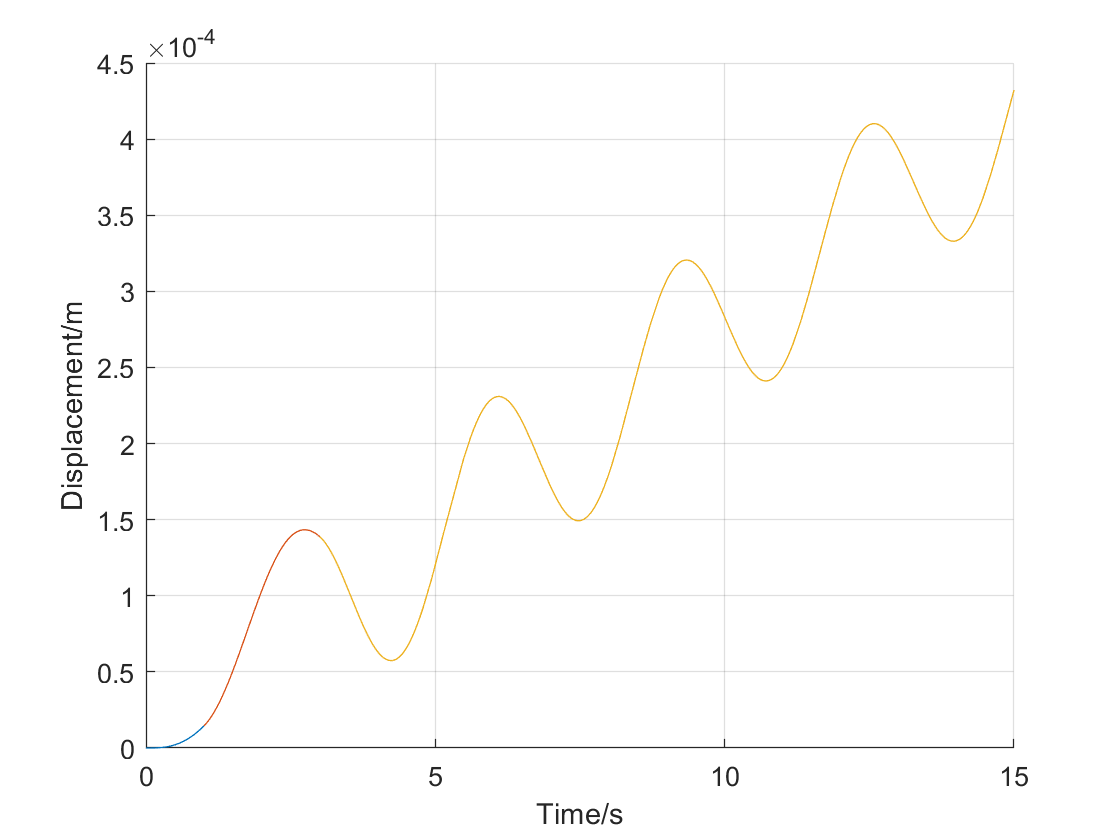
\includegraphics[width = 0.75\textwidth]{./img/q1e.png}
    \caption{Response of sensor.}
\end{figure}
\section{Linear modelling}
\subsection{Description of non-linearity between $y(t)$ \& $\theta(t)$}
The following function:
\begin{equation}
    \frac{\dif y\left( t\right)}{\dif t} = 150 \cos \left(\theta\left(t\right)\right) - 47
\end{equation}
has a non-linear relationship due to $\theta(t)$ being within a cosine function. There is also an offset value of $47$ which makes our relationship non-linear as well.
\subsection{Description of non-linear relationship in a real system}
An example of a non-linear relationship is car velocity and air resistance. Our input is the velocity of the car and our output is the drag force We can describe this relationship with the following equation.
\begin{align}
    F_D & = \frac{1}{2} \rho v^2 C_D A \\
    F_D & \propto v^2
\end{align}
The relationship between the drag force and velocity is proportionally squared. This means that as velocity increases, our drag force will increase by four times. Non-linearity can also come in the form as headwind or tailwind. Mathematically, this would be represented as a constant term ($B$) added to our equation. For example:
\begin{equation}
    F_D = \frac{1}{2} \rho v^2 C_D A + B\\
\end{equation}
\section{Linear model performance and stability}
\subsection{Unstable process + description of actuator switching on}
The transfer function, $G_p(s)$ is:
\begin{equation}
    G_p (s) = \frac{Y(s)}{V(s)} = \frac{1}{\left(s^2 - 81\right)}\frac{k}{\left(0.05s + 1\right)}
\end{equation}
By looking at the position of the roots ($s = 9$, $s = -9$, $s = -20$), we can check whether our system is unstable. We have a root at $s = 9$, which is on the positive side of the s-plane. This means that our whole system is unstable.

Our poles lie on the real axis on the positive side of the s-plane. Hence, when we switch our voltage to \SI{5}{\volt}, we will find that our rudder angle will exponentially rise. We will not see any oscillation as our response will have no sine term. The rudder angle will continually to increase until it reaches its mechanical limit and potentially damage itself. The rudder angle may go in either direction (positive or negative/left or right) until it reaches this limit.
\subsection{Root locus and effect of proportional control}
Using the following MATLAB code, the root locus of the system was plotted in Figure \ref{q3b}.
\lstinputlisting{./mCode/q3b.m}
\begin{figure}[H]
    \centering
    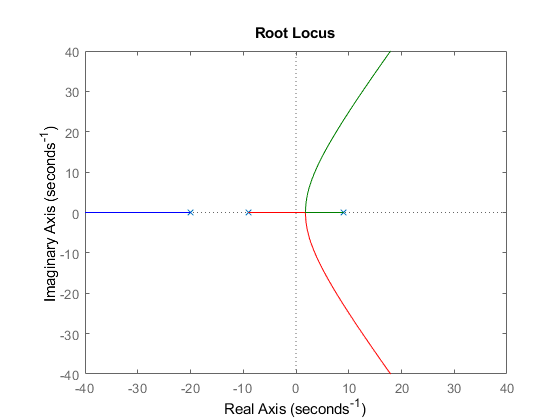
\includegraphics[width = 0.75\textwidth]{./img/q3b.png}
    \caption{Root locus of system.}
    \label{q3b}
\end{figure}
This root locus diagram shows us that the system would be unstable in closed-loop operation for all possible values of gain $K$, hence rendering proportional control ineffective for stabilising the system.
\subsection{Negative velocity feedback controller}
\subsubsection{Plot of root locus}
Our new transfer function is:
\begin{equation}
    H_p(s) = \frac{k\left(s+8\right)}{0.05s^3 + s^2 -4.05s - 81}
\end{equation}
Using the following MATLAB code, the root locus of the system was plotted in Figure \ref{q3ci}.
\lstinputlisting{./mCode/q3ci.m}
\begin{figure}[H]
    \centering
    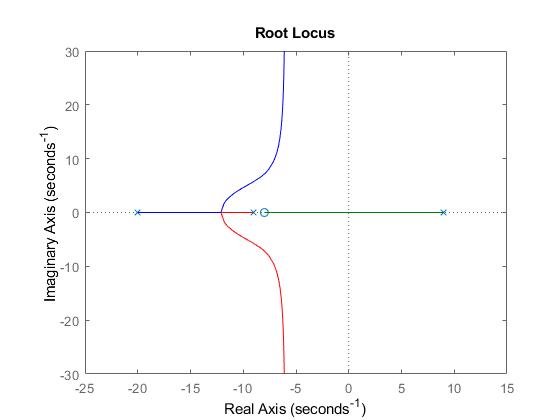
\includegraphics[width = 0.75\textwidth]{./img/q3ci.png}
    \caption{Root locus of system with negative velocity feedback controller.}
    \label{q3ci}
\end{figure}
\subsubsection{Areas where damping ratio is higher than 0.6 + damped natural frequency is higher than \SI{7}{\radian\per\second}}
We are given that our damping ratio must be at least 0.6 and that our damped natural frequency must be at least \SI{7}{\radian\per\second}:
\begin{gather}
    \zeta \geq 0.6\\
    \omega_d \geq 7
\end{gather}
Solving to find the minimum undamped natural frequency:
\begin{gather}
    \omega_n = \frac{\omega_d}{\sqrt{1 - \zeta^2}}\\
    \omega_n = \frac{7}{\sqrt{1-0.6^2}}\\
    \omega_n = 8.75
\end{gather}
Since the undamped and damped natural frequency are proportional, we know that:
\begin{equation}
    \omega_n \geq 8.75
\end{equation}
Using the following MATLAB code, the regions which fulfil the above constrains were plotted in Figure \ref{q3cii}.
\lstinputlisting{./mCode/q3cii.m}
\begin{figure}[H]
    \centering
    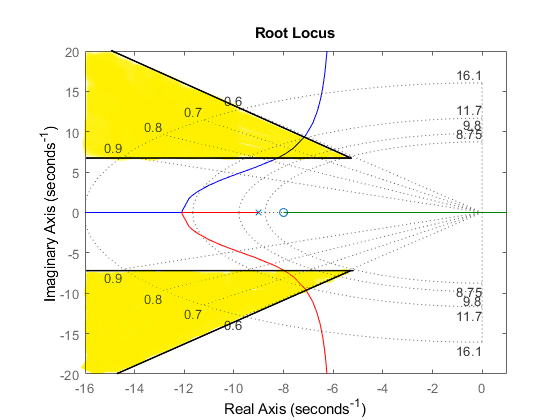
\includegraphics[width = 0.75\textwidth]{./img/q3cii2.png}
    \caption{Regions on root locus diagram where $\zeta \geq 0.6$ and $\omega_d \geq 7$.}
    \label{q3cii}
\end{figure}
\subsubsection{Range of $k$ where performance specifications are achieved}
By inspecting our MATLAB plots, we can find the gain values at any specified point.
\begin{figure}[H]
    \centering
    \begin{minipage}{.5\textwidth}
        \centering
        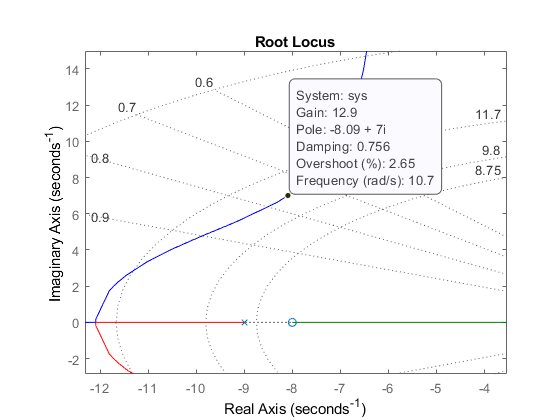
\includegraphics[width = \linewidth]{./img/q3ciii1.png}
        \caption{Minimum $k$ value.}
        \label{q3ciii1}
    \end{minipage}%
    \begin{minipage}{.5\textwidth}
        \centering
        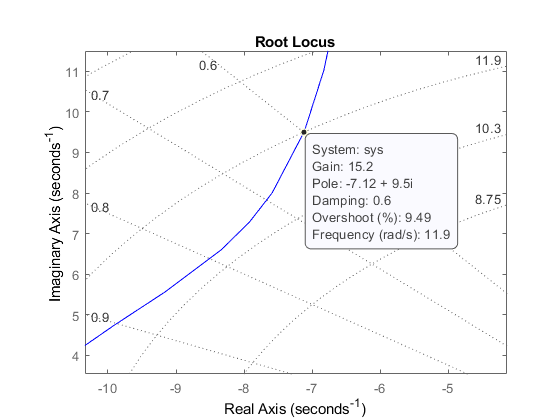
\includegraphics[width = \linewidth]{./img/q3ciii2.png}
        \caption{Maximum $k$ value.}
        \label{q3ciii2}
    \end{minipage}
\end{figure}
Here, we find that the maximum gain value that we can have is 15.2 at pole value $-7.12 + 9.5i$, limited by our damping ratio. For gains below 15.2, our pole position moves towards the real axis and away from the imaginary axis. The minimum gain value we can have is limited by the damped natural frequency and at a pole value of $-8.09 + 7i$, our gain is 12.9. Therefore:
\begin{equation}
    12.9 \leq k \leq 15.2
\end{equation}
\section{Controller techniques}
\subsection{Description of closed loop position control system}
The system I have chosen to describe is a drone autopilot system. The drone I have picked as part of this analysis is a DJI Mavic 3. This drone is used to take high quality aerial video footage, hence stability and control are important for this particular drone. In a simple case, let us try and make our drone hover in a fixed position above the ground (in a fixed reference frame). Our desired output response is to keep the drone's coordinates fixed. To further simplify our example, let us only consider the motion in the $z$-axis (altitude).

The actuator is the motors attached to the drone propellers. The physical position to be controlled is the altitude of the drone. According to the drone specifications, the drone has a hovering accuracy range of $\pm\SI{0.1}{\metre}$ in the vertical (with Vision Positioning). Using GPS data, we have a lower hovering accuracy at $\pm \SI{0.5}{\metre}$ \citep{dji}. As this is a video recording drone, the ability to stay at a fixed altitude and to not `drift' is important to prevent the footage from looking shaky/blurry/distracting.
\subsection{Specify disturbances}
As the ground which the drone flies above is rough, we will find that there are perturbations, peaks and valleys in the terrain. In order to determine the distance to the ground, we have to measure the instantaneous vertical distance from the drone to the ground.

Some disturbances our drone will experience is wind, changing its position in the air. This will manifest as noise as the position of the drone will always be changing. Control is needed to keep the drone in a fixed position.

The DJI Mavic 3 uses GPS to determine its distance from the ground \citep{dji}. If the drone is using GPS to determine its distance from the ground, there will be measurement noise. This will come from the signal power varying (the signal gain of the radio signals used to communicate with GPS satellites), the method of analog-to-digital conversion will produce signal noise, and the design of the antennas will also produce signal noise. The position data from the GPS receivers then needs to be processed and denoised, in order for an accurate measurement to be made. The position data then needs to be referenced against pre-existing terrain data. This terrain data should have a resolution high enough to accurately determine the distance to the ground over any point, but also the data should be processed to be `smooth'. Details such as rocks/small boulders or trees do not necessarily have to be in the terrain data, as the drone also uses Vision Positioning to determine the distance to smaller objects at closer distances \citep{dji}.
\section{Inverted pendulum}
\subsection{Identification and description of assumptions and limitations for the model of a rotary inverted pendulum}
For the inverted pendulum system, we are considering the angle to be small. Hence, we can use the small angle approximation:
\begin{equation}
    \sin \theta \approx \theta
\end{equation}
Next, we have constrained our pendulum to only move in a 2D-plane ($x$- and $z$- axes), simplifying our model. We can make further simplifications by neglecting frictional forces and drag acting on the pendulum during movement.
\subsection{Moving rocket to final position}
There are a few steps to steering the rocket to minimise the $x$-position.
\begin{enumerate}
    \item The rocket is vertical but a distance $x$ from the centre of the base.
    \item Let us first gimbal our engine to produce a thrust which will move the base of the rocket to the right. This will happen if we gimbal the engine to the left.
    \item Now the centre of mass of the rocket is to the left of the long axis and it will start to move.
    \item Now we can gimbal our engine in-line with the long axis of the rocket, and our rocket will start to translate left.
    \item When we have reached the $x = 0$ position, we can gimbal our engine to the right, which will move the centre of mass back in line with long axis of the rocket and the engine, straightening out our rocket.
    \item Rocket is stable and stationary above the pad.
\end{enumerate}
\begin{figure}[H]
    \centering
    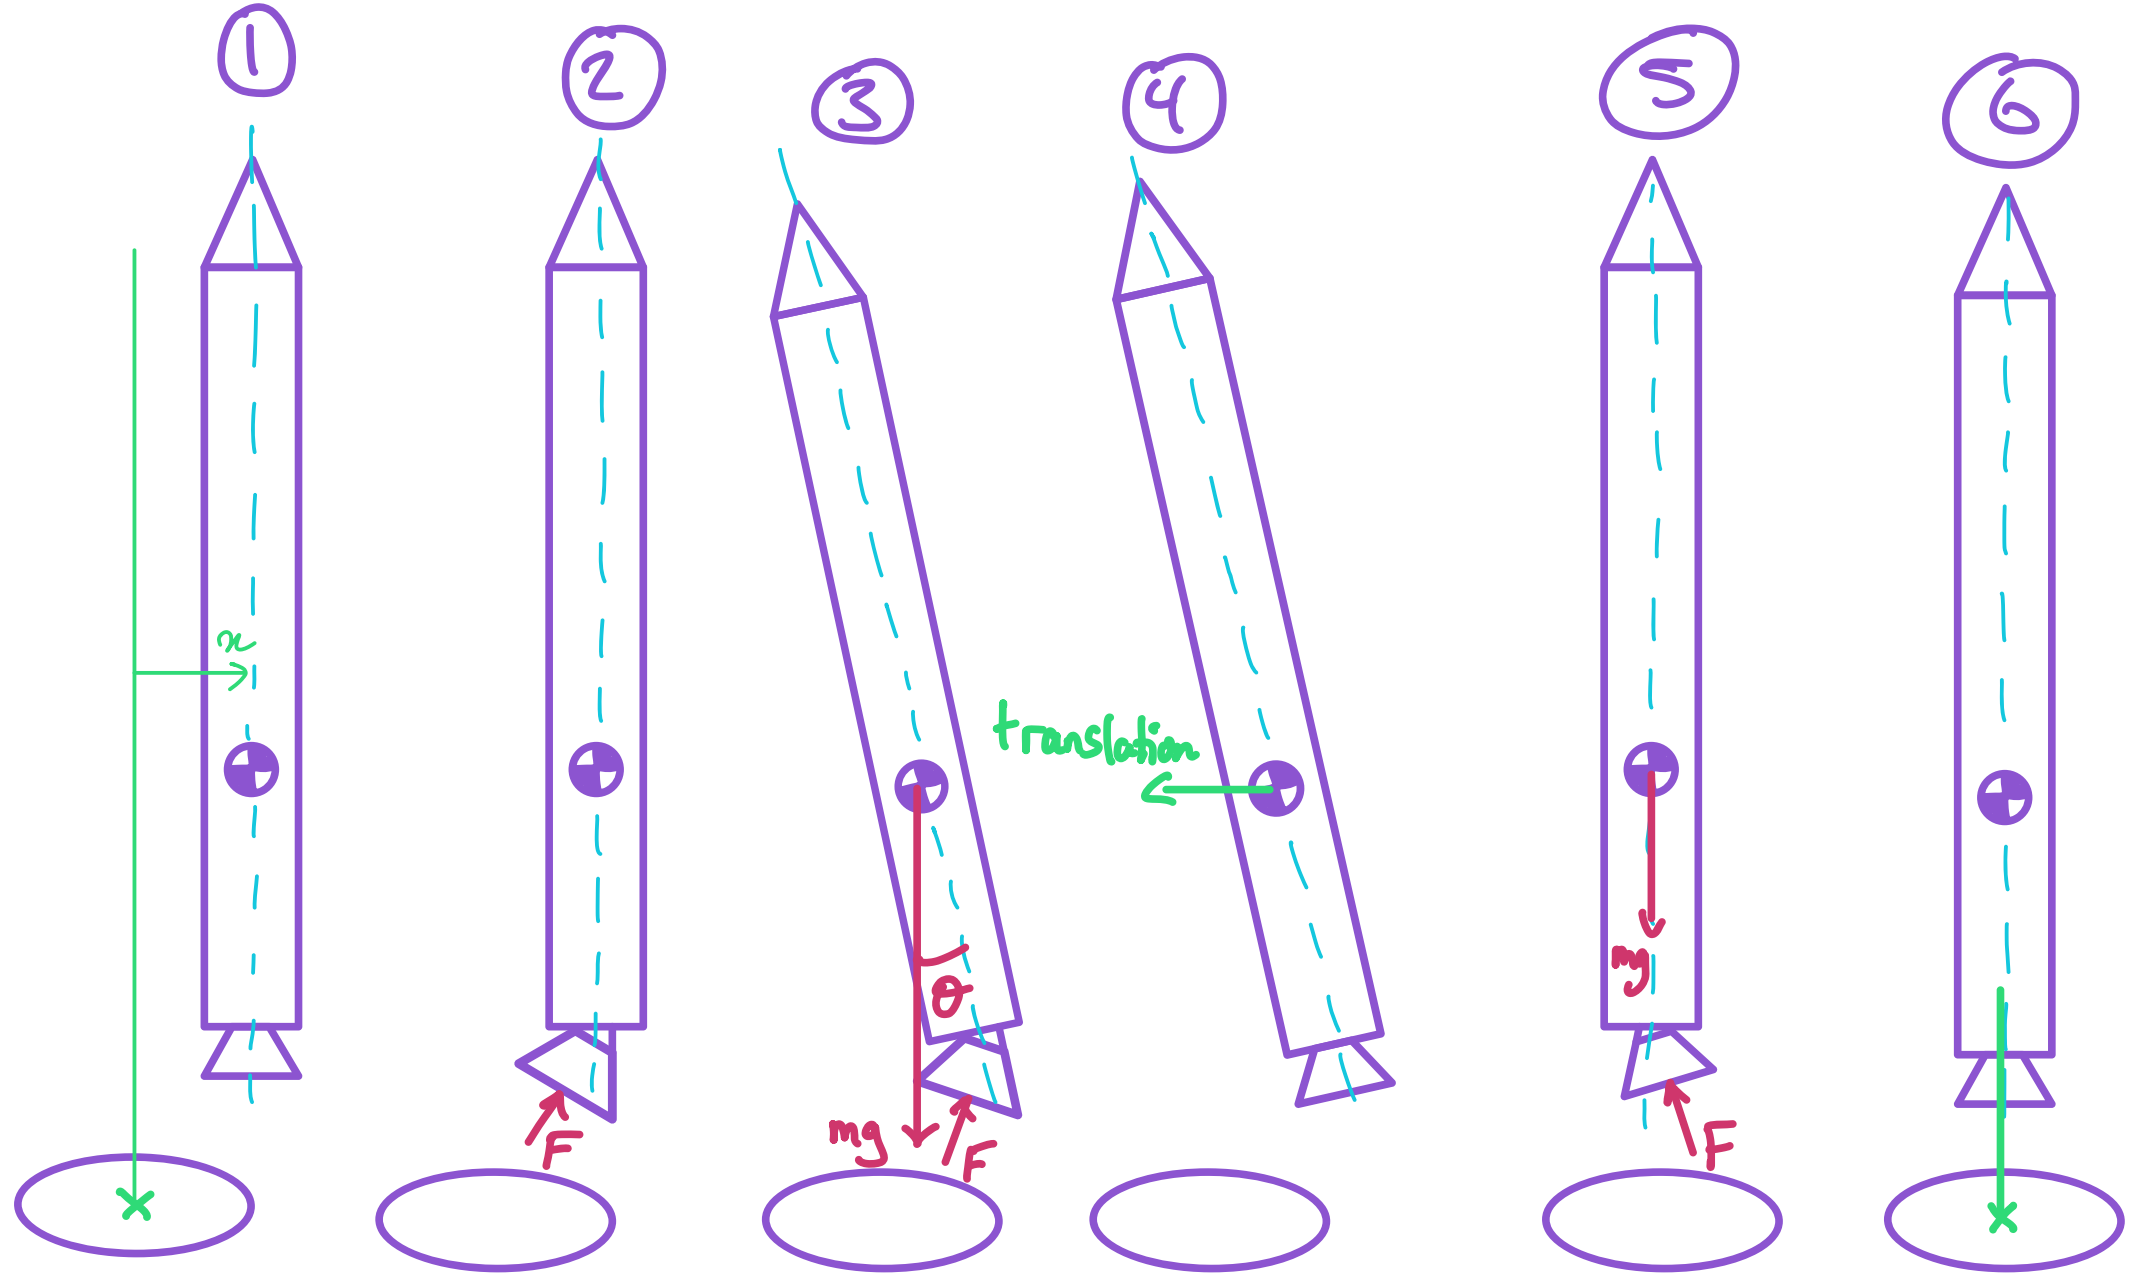
\includegraphics[width = \textwidth]{./img/q5b.png}
    \caption{Stages of rocket aligning with base pad.}
    \label{q5b}
\end{figure}
\section{Multi-Degree-of-Freedom systems}
\subsection{Example of a system with multiple degrees-of-freedom}
The system that I have chosen to describe is a hydraulic vehicle suspension system. This system's primary purpose is to reduce transmitted vibrations from the road surface to the car body and maximise tyre contact with the ground. It can achieve different characteristics by utilising oil or compressed air to change the stiffness and damping of the system. In one model, we can model the system as such:
\begin{figure}[H]
    \centering
    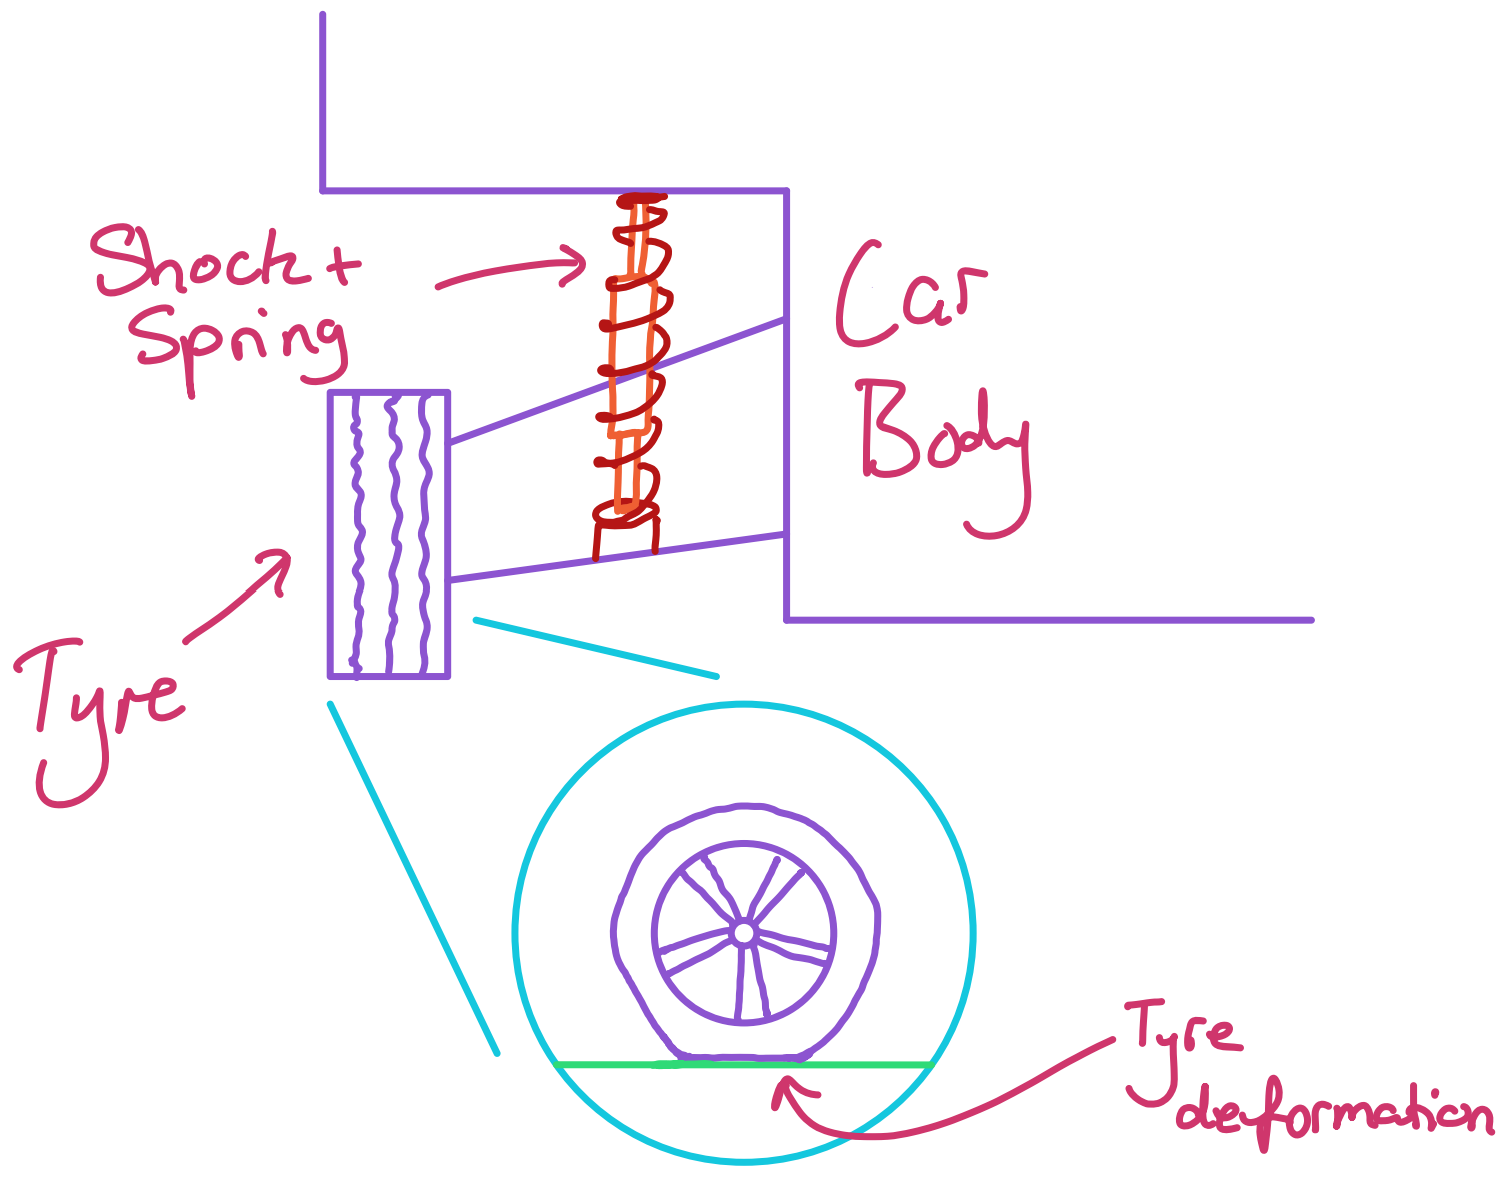
\includegraphics[width = 0.5\textwidth]{./img/q61.png}
    \caption{Physical model of suspension system.}
    \label{q61}
\end{figure}
\begin{figure}[H]
    \centering
    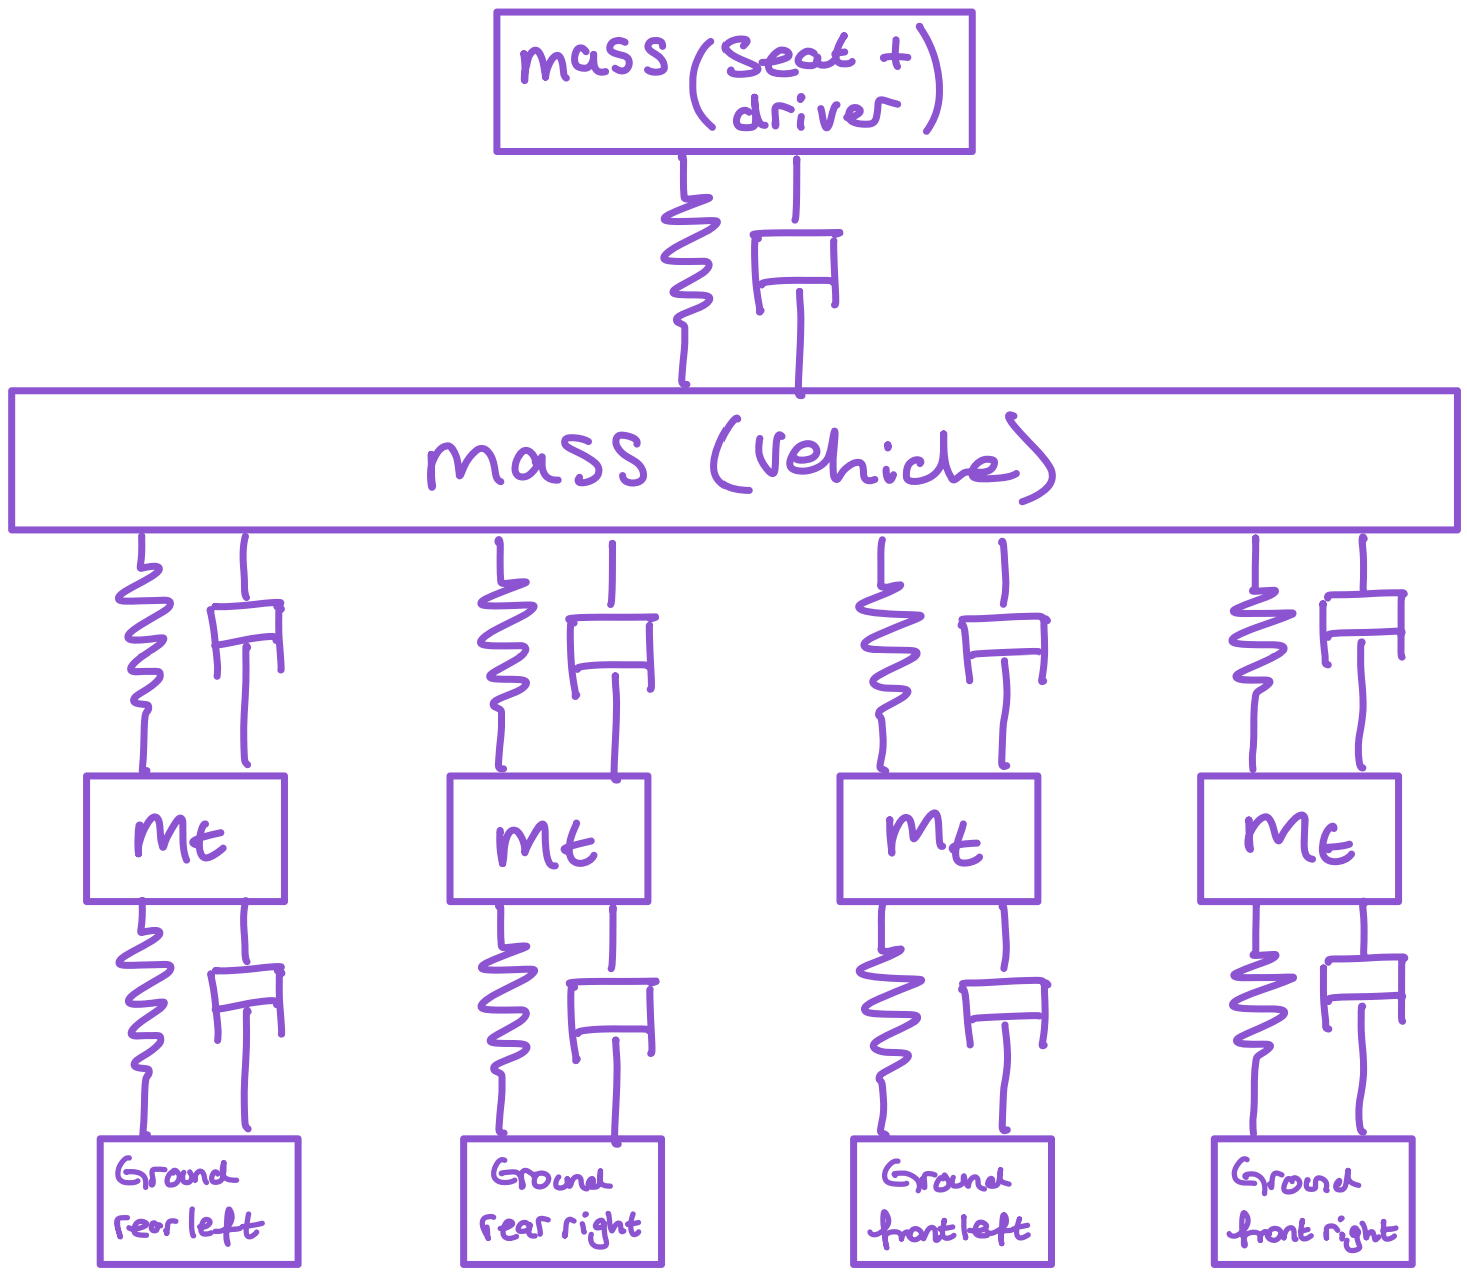
\includegraphics[width = 0.5\textwidth]{./img/q62.png}
    \caption{Model of MDOF system.}
    \label{q62}
\end{figure}
Our inputs are forces applied (and hence motion relative to the rest of the system) to the tyres from the ground. We know that tyres themselves have a certain stiffness and certain deformation characteristics, which can be modelled.

The output of our system is the overall displacement of the driver sitting in the car. We could model each individual component from the ground to the driver separately, but for simplicity's sake, the seat and driver have been modelled as one system (the seat is directly attached to the frame of the vehicle).

The forces transmitted from the ground can vary due to perturbations in the road surface, its smoothness and any obstacles in the path of the tyre. The ground may also not be homogeneous and each wheel may be receiving different displacements (for example on off-road terrain). Another external influence could be weather and damage to the components. Rainy/snowy weather would affect how the tyres interact with the ground, possibly preventing a good contact between tyre and ground. Damage to the components could be failed shocks/bushings (dampers) or corroded bolts. These would result in components being able to move in ways in which vibrations could be transmitted through the car in unwanted ways.

In vehicle suspension systems, the springs and shocks are not directly connected to the tyres, instead they are connected to the (lower) control arms. Similarly, the vehicle is a large object and the suspension struts are connected in the corners of the car, whereas the driver sits (roughly) in the middle of the vehicle. The flexure and stiffness of the car body may be negligible in this case, we may also consider the flexure in the control arms to be negligible as they are rigid components.

The main sensors would be a suspension spring displacement sensor and an accelerometer placed on the car body. This will give the onboard computer information about how the tyre is deforming and how the car body is reacting. There may be a supplementary sensor installed in the car seat to fine tune the response of the hydraulic suspension. Certain programmes can be installed on the computer which can tell the hydraulic suspension components to either stiffen or relax the damping within the shocks. This would have the effect of improving vehicle handling for a variety of scenarios. For example, for a high-performance scenario, a stiffer suspension system would allow for the tyres to have a better contact patch with the ground, allowing more power to be transmitted to the ground from the engine. On the other hand, a relaxed suspension system would smoothen out and reduce vibrations from the ground as experienced by the driver.

The controller to be used in this case would have to utilise some form of PID control. Proportional control would be used to control the vehicle vibrations (displacement). Integral control would be used to keep the vehicle stable after oscillatory action. This could be in the form of stabilising the ride height (distance between car body and ground) of the vehicle after a large displacement. Derivative control would be needed to prevent large overshoots, which would result in an overly `bouncy' suspension response, with many oscillations after an initial displacement. Together, proportional, integral and derivative control would be necessary to stabilise the car body from the various forces exerted upon it by the road through the tyres.
\bibliographystyle{agsm}
\bibliography{references}
\end{document}